%RESULTS
\chapter{Results}
In this chapter we will present the outcome of this project in the form of test
results, AST output, and error handling capabilities.

\section{Tests}
\subsection{Unit tests}
Unit testing was used solely for regression testing, so they did not directly 
produce any results of particular interest.

\subsection{Manual tests}
To test for standards compliance, we created a manual test harness for running
the complete XQuery Test Suite\cite{w3c05} consisting of 12584 queries. Our
initial tests showed a 54\% coverage (6846 queries successfully parsed), and
after additional improvement and calibration ..

//TODO!



% PARSER OUTPUT
\section{Parser output}
\subsection{Abstract syntax trees}
\label{sect:results:parser_output:ast}

% Implementation: error handling
\section{Error Handling}
\label{sec:impl:errorhandling}
\begin{figure}[!h]
  \centering
    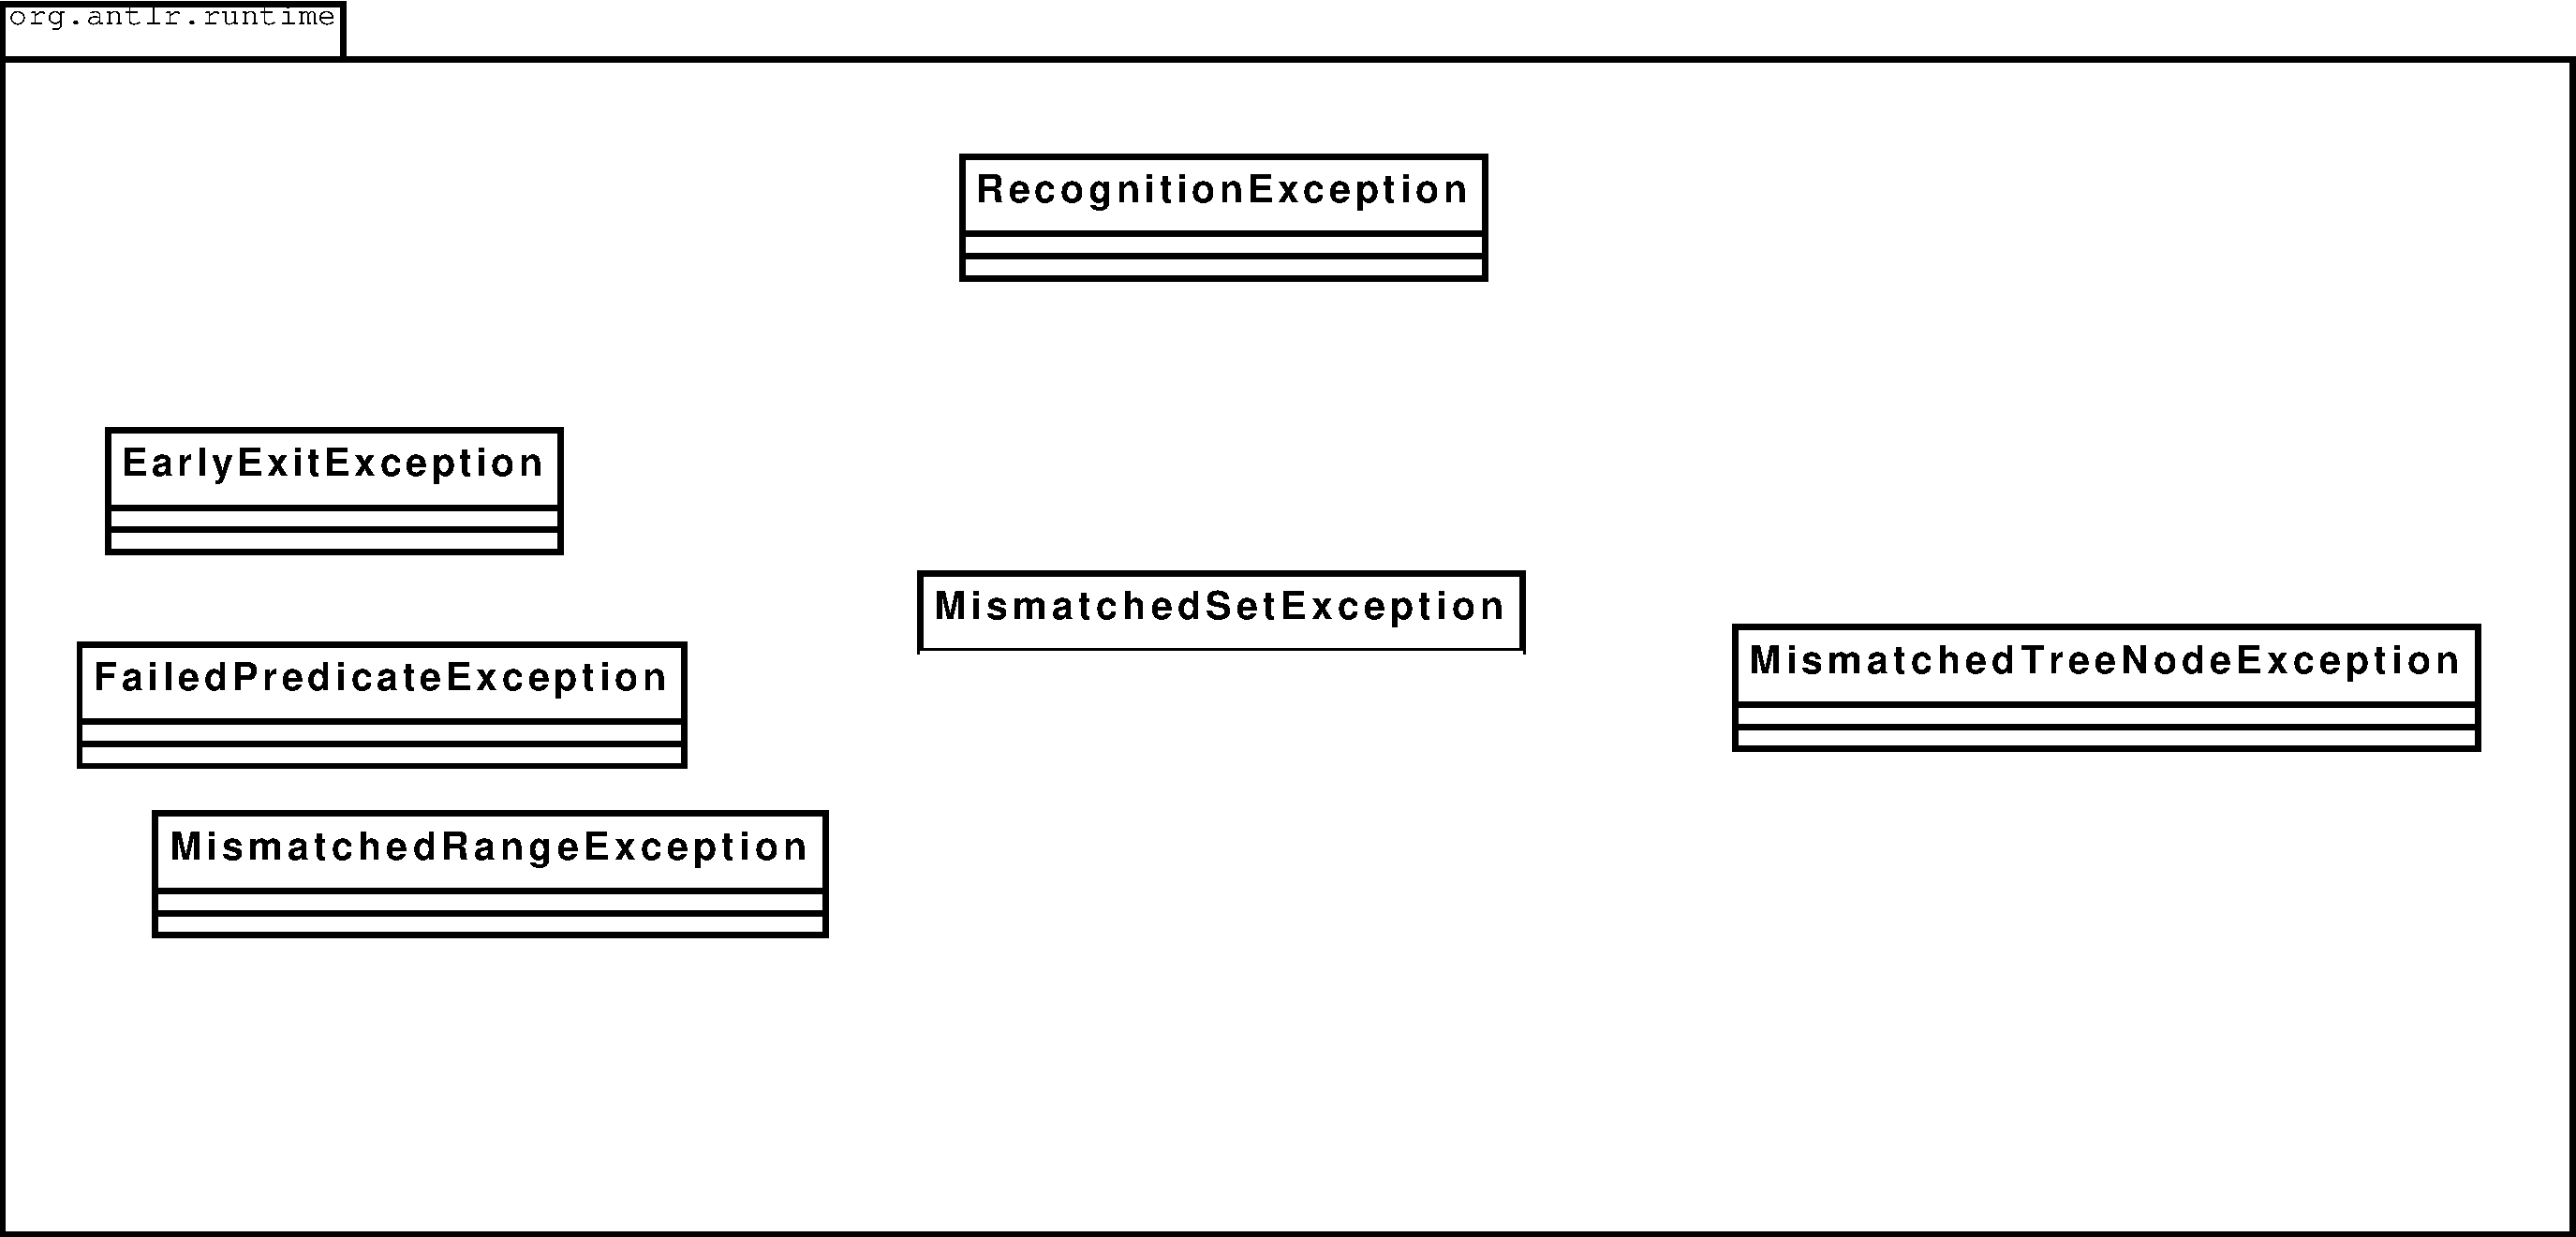
\includegraphics[width=1\textwidth]{diagrams/exception_uml}
  \caption{ANTLR exceptions class hierarchy}
\label{fig:antlrException}
\end{figure}
Error handling in ANTLR is initially done by catching exceptions and printing
an error message to stderr. The parser will then attempt to recover from the
error and continue parsing. This behaviour is not always desirable, so certain
methods were overridden to allow exceptions to be thrown upwards the stack to
the program that initiated the parser (the calling program, or top-level
program). An overview of the posible exceptions ANTLR can throw is shown in figure \ref{fig:antlrException}.

Specifically, this was done by overriding the methods \verb!mismatch()! as well as
\verb!recoverFromMismatchedSet()!, as such:

\begin{Verbatim}
    protected void mismatch(IntStream input, 
                            int ttype, 
                            BitSet follow)
        throws RecognitionException
    {
        throw new MismatchedTokenException(ttype, input);
    }

    public void recoverFromMismatchedSet(IntStream input, 
                                         RecognitionException e, 
                                         BitSet follow)
        throws RecognitionException
    {
        throw e;
    }
\end{Verbatim}

Additionally, a special \verb!@rulecatch! rule had to be added to force ANTLR from
handling errors and instead throwing the exceptions upwards:

\begin{Verbatim}
@rulecatch {
    catch (RecognitionException e) {
        throw e;
    }
}
\end{Verbatim}

However, some exceptions thrown by the lexer were impossible to handle - these
were handled in the \verb!nextToken()! method in the \verb!Lexer! superclass.
This issue has been documented in section 
\ref{sect:error_handling:syntax_errors}.


\section{Summary}
In this chapter we have presented the essential resulting output from this
project. First we presented our test results, noting that we started out at   
54\% coverage which increased to 88\% after tweaking the parser somewhat.
Conformity of the parser (or, in some unfortunate cases, the lack thereof) is
further  discussed in section \ref{sect:future:knownBugs}. The coverage test
results are also further discussed in section
\ref{sect:discussion:coverageResults}.

Further we proposed some possible AST structures as generated by our parser, in
particular FLWOR constructs, path expressions, function declarations, and
full-text operations. However, these propositions are not definitive, and it
will take further research and possibly a ``trial-and-error'' approach to settle
on optimal AST structuring.

Finally we presented the error handling implemented in our parser, and some
possible problems with the current implementation. 

In the next chapter we will further elaborate on these issues and discuss
possible solutions.